\subsection{Circuito RLC}\label{sec: RLC}
\paragraph{}
En esta sección, se estudió la respuesta del circuito RLC conformado en la figura \ref{esq: RLC}, conectando en serie un resistor de resistencia variable, un capacitor de $C=\SI{9.39(0.07)e-9}{F}$ y un inductor de $L=\SI{999(9)e-3}{H}$. Se alimentó al sistema con una fuente de ondas cuadradas de tensión $V_0=\SI{4.96(0.15)}{V}$ Se analizaron experimentalmente los casos subamortiguados (sección \ref{sec:RLC sobre}) y sobreamortiguados (sección \ref{sec:RLC sub}) modificando la resistencia $R$ según los valores dados por las condiciones en \eqref{eqn:condicion sobre} y \eqref{eqn:condicion sub}.

\subsubsection{Caso sobreamortiguado}\label{sec:RLC sobre}
\paragraph{}
Para estudiar el caso sobreamortiguado, se registró con un osciloscopio la respuesta del sistema para $R_{sobre}=\SI{30.37(0.03)e3}{\Omega}$. Esta resistencia cumple con la condición dada en \eqref{eqn:condicion sobre} para los valores de $C$ y $L$ utilizados. Se realizó un ajuste de la caída de tensión en el resistor con respecto al tiempo con la ecuación \eqref{eqn:RLCsobre} y se obtuvo el gráfico de la figura \ref{fig:RLC sobreamortiguado}, que muestra el ajuste con sus respectivos residuos.

\begin{figure} [H]
    \centering
    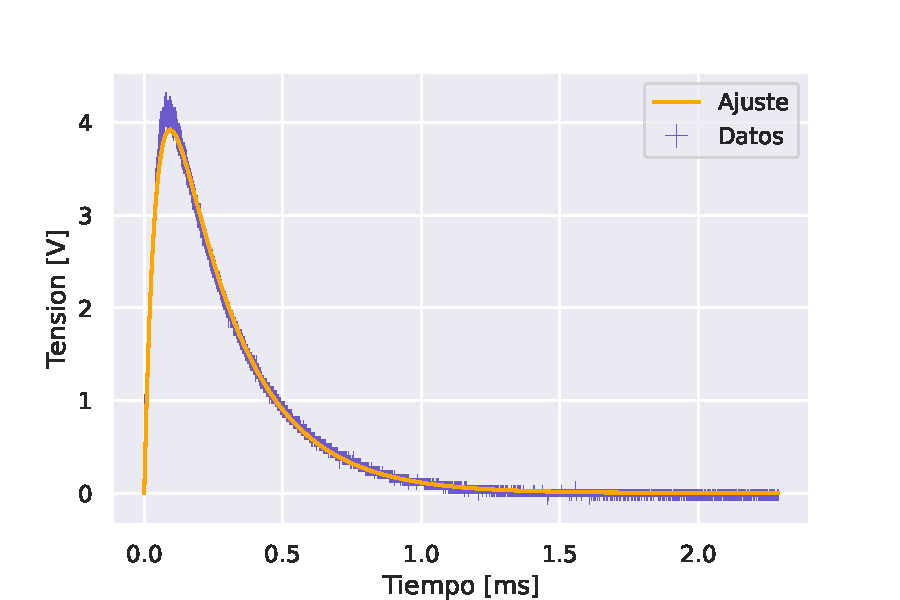
\includegraphics[scale=0.5]{Figuras/RLC/RLC sobreamortiguado 1.pdf}
    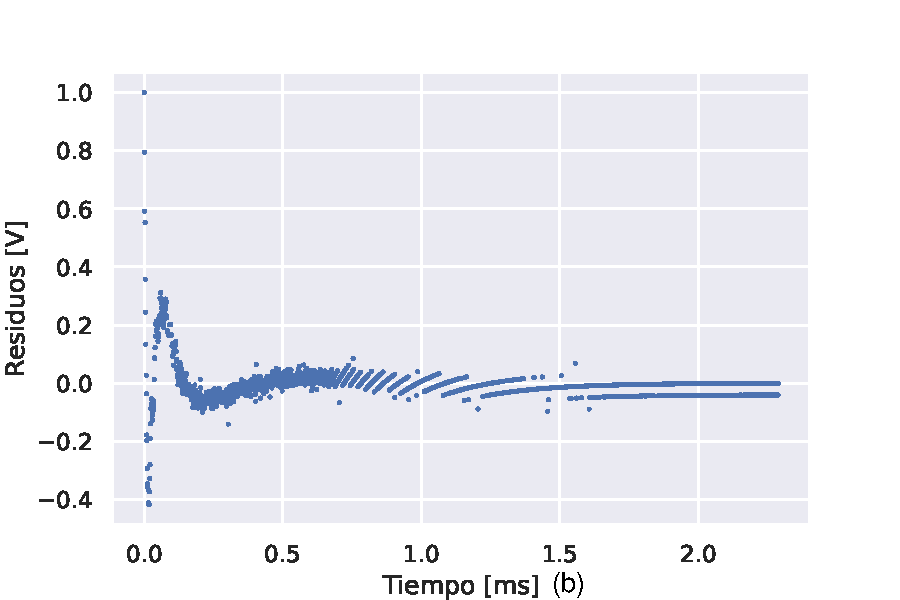
\includegraphics[scale=0.5]{Figuras/RLC/residuos sobreamortiguado.pdf}
    \caption{Caso sobreamortiguado del circuito RLC, con $R_{sobre}=\SI{30.37(0.03)e3}{\Omega}$. En (a), los datos y el ajuste con la ecuación \eqref{eqn:RLCsobre}. En (b), los residuos del ajuste en azul.}
    \label{fig:RLC sobreamortiguado}
\end{figure}
\paragraph{}
Con el ajuste, se obtuvieron valores de $L = \SI{1.18(0.02)}{H}$, $R = \SI{30.5(0.5)e3}{\Omega}$ y $C = \SI{9.4(0.4)e-9}{F}$, lo cual es consistente con lo medido independientemente para la inductancia, resistencia y capacitancia. También se calculó $V_0 = \SI{4.94(0.04)}{V}$, que no presenta diferencias significativas con el valor reportado previamente. Sin embargo, como se puede observar en la figura \ref{fig:RLC sobreamortiguado} (b), los residuos del ajuste presentan una distribución no aleatoria, particularmente durante las primeras décimas de milisegundo. Entonces debe considerarse la posibilidad de que existan factores que no se hayan tenidos en cuenta. Esto puede ser apreciado con mayor claridad al aumentarse la resistencia total del sistema. Con $R =\SI{2.0(0.1)e6}{\Omega}$, el resultado es el que muestra a la figura \ref{fig:falopa}.
\begin{figure} [H]
    \centering
    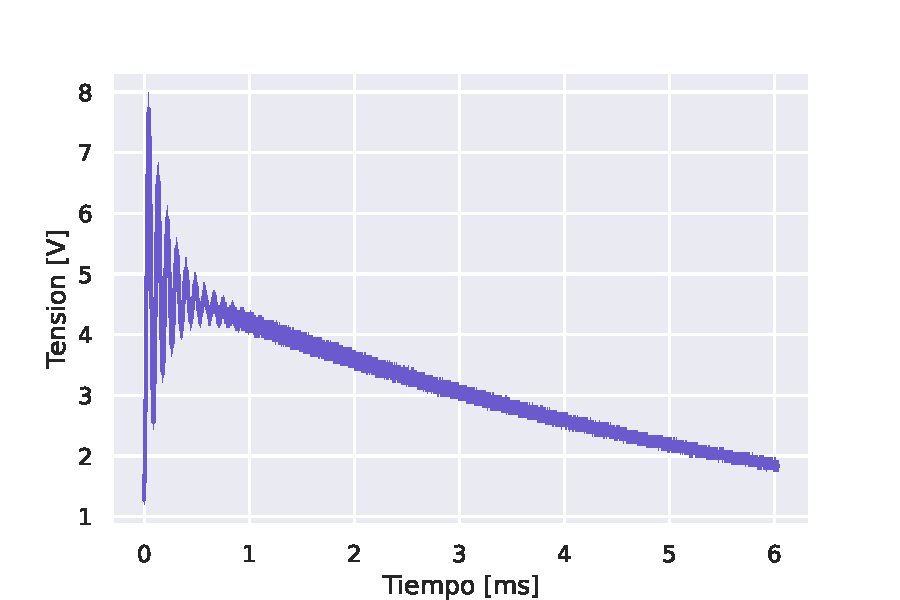
\includegraphics[scale=0.7]{Figuras/Falopa/falopa.pdf}
    \caption{Tensión en función del tiempo para $R=\SI{2.0(0.1)e6}{\Omega}$.}
    \label{fig:falopa}
\end{figure}
\paragraph{}
Como se puede apreciar en la figura \ref{fig:falopa}, al aumentar la resistencia aparece una oscilación montada sobre la curva del sobreamortiguado, cuya frecuencia es mucho mas grande (Aproximadamente seis veces mas grande) que la frecuencia observada con el mismo circuito en el régimen subamortiguado. Sin embargo, es esperable que el modelo no funcione para estos valores de resistencia ya que la resistencia de el osciloscopio es de $1M\Omega$\cite{manual_osciloscopio} coincidiendo en orden de magnitud con las resistencias a las cuales aparece este fenómeno. Por lo tanto, la aproximación de voltímetro ideal implícita en el razonamiento previo ya no es valida para estos valores de resistencia. Por lo tanto, se considera una hipotesis razonable el hecho de que la capacidad e inductancia interna del osciloscopio actue como un circuito RLC serie y esa sea la causa de las desviaciones del modelo observadas.

%-------------------------------------------------------


\subsubsection{Caso subamortiguado}\label{sec:RLC sub}
\paragraph{}
Para el estudio del caso subamortiguado, se registró la tensión para dos resistencias, $R_1=\SI{1365(2)}{\Omega}$ y $R_2=\SI{866(2)}{\Omega}$. Estas resistencias cumplen con la condición dada en \eqref{eqn:condicion sub}. Se realizó un ajuste de la caída de tensión en el resistor con respecto al tiempo con la ecuación \eqref{eqn:RLCsub}. Para $R_1$, se obtuvo el gráfico de la figura \ref{fig:RLC subamortiguado 1}. Este caso es sustancialmente diferente al sobreamortiguado dado que presenta una oscilación, antes inexistente debido al uso de grandes resistencias respecto a L y C.

\begin{figure} [H]
    \centering
    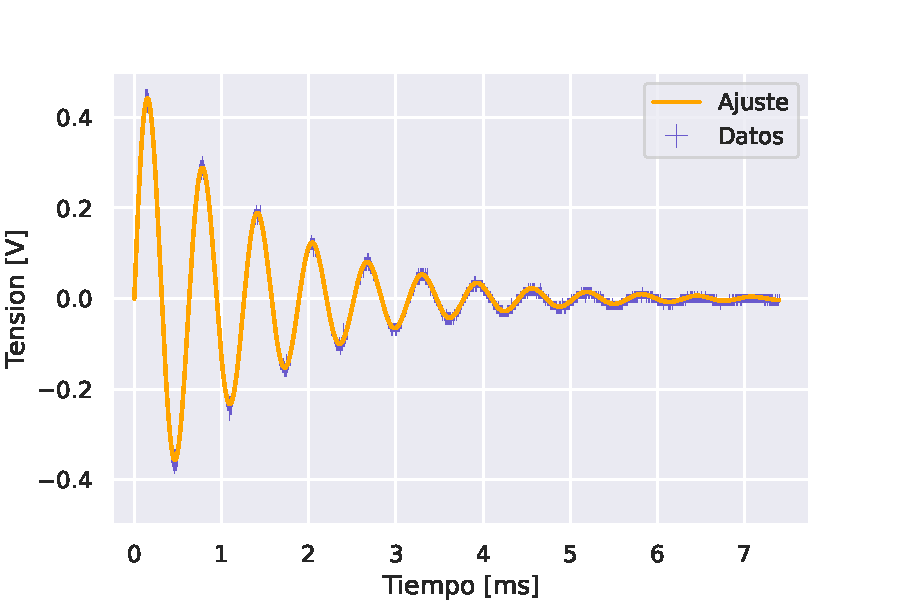
\includegraphics[scale=0.7]{Figuras/RLC/RLC subamortiguado 1.pdf}
    \caption{Tensión en función del tiempo para el circuito RLC con $R_1 = \SI{1365(2)}{\Omega}$. Se observa la tensión oscilando con $\omega = \SI{1.00(2)e4}{\frac{rad}{s}}$, cuyo módulo decae exponencialmente. Los residuos del ajuste no muestran }
    \label{fig:RLC subamortiguado 1}
\end{figure}
\paragraph{}
En este caso, se obtuvo una inductancia de $L = \SI{1.0(0.2)}{H}$, una $C = \SI{10(2)e-9}{F}$ y un $\omega = \SI{1.00(2)e4}{\frac{rad}{s}}$. Estos resultados no varían significativamente con los valores de $L$ y $C$ medidos directamente. 
\paragraph{}
Para $R_2$, se obtuvo el gráfico de la figura \ref{fig:RLC subamortiguado 2}.  
\begin{figure} [H]
    \centering
    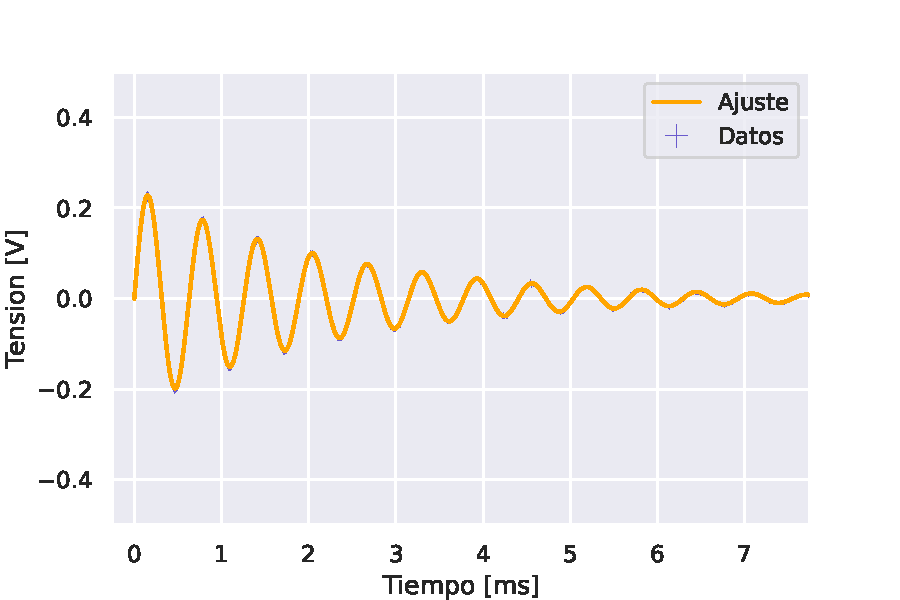
\includegraphics[scale=0.7]{Figuras/RLC/RLC subamortiguado 2.pdf}
    \caption{Tensión en función del tiempo para el circuito RLC con $R_2$. }
    \label{fig:RLC subamortiguado 2}
\end{figure}
\paragraph{} 
Se obtuvo una inductancia de $L = \SI{1.0(0.3)}{H}$, una $C = \SI{10(3)e-9}{F}$ y un $\omega = \SI{1.00(3)e4}{\frac{rad}{s}}$. Al igual que en el primer caso, los resultados no varían significativamente con los valores de $L$ y $C$ medidos directamente. Estos resultados son coherentes dado que al utilizar dos resistencias distintas, $(R_2 < R_1)$, se espera que con una resistencia mayor se obtenga un decaimiento de tensión mayor. 